\documentclass{scrartcl}
\usepackage[ngerman]{babel}
\usepackage{amsmath}
\usepackage{graphicx}
\usepackage{float}
\usepackage{xcolor}
\usepackage{mhchem}
\usepackage{siunitx}
%\usepackage{circuitikz}
\title{Zusammenfassung Einführung in die Physik Teil 2}

\begin{document}

\maketitle
\tableofcontents
\newpage



\section{Elektrostatik}
Ladungen sind immer an Teilchen mit einer Masse gebunden. Ein Ladungstransport stellt einen elektrischen Strom dar und Ladungstransport
ist immer mit Massentransport verbunden.
\begin{itemize}
\item negative Ladungen: Elektronen, negative Ionen 
\item positive Ladungen: Protonen, positive Ionen
\end{itemize}
Gleichartige Ladungen stoßen sich ab, entgegengesetzte Ladungen ziehen sich an. Alle Kräfte zwischen Atomen und Molekülen,
Festkörpern haben ihren Ursprung in Ladungen.\\

Die elektrische Ladung $q$ hat die Einheit Coulomb (SI-Einheit):
\begin{align}
    [q]=1\,\mathrm{C}=1\,\mathrm{A\,s}
\end{align}
Die Elementarladung $e$ hat den Wert:
\begin{align}
    e=1,6021892(46)\times 10^{-19}\,\mathrm{C}
\end{align}
Das Verhältnis der Elementarladung zur Masse eines Elektrons beträgt:
\begin{align}
    \frac{e}{m_\mathrm{e}}=1,7588047(49)\times 10^{11}\,\frac{\mathrm{C}}{\mathrm{Kg}}
\end{align}
Daraus folgt, dass die Masse eines Elektrons deutlich kleiner ist als der Wert der Elementarladung.
Die Ladung der Quarks ist ein Vielfaches der Ladung eines Protons/Elektrons und somit der Elementarladung.
\begin{align}
    q_\mathrm{up\, Quarks}&=\frac{2}{3}q_\mathrm{Proton}=\frac{2}{3}e\\
    q_\mathrm{down\, Quarks}&=\frac{1}{3}q_\mathrm{Elektron}=-\frac{1}{3}e
\end{align}
Die Ladung eines Protons ist gleich der Elementarladung und die Ladung eines Elektrons gleich der negativen Elementarladung.
\begin{align}
    q_\mathrm{Proton}=-q_\mathrm{Elektron}
\end{align}

\subsection{Ladungserhaltung}
In einem abgeschlossenen System bleibt die Gesamtladung zeitlich konstant, das heißt Ladungen können
werder erzeugt noch vernichtet werden. Es gilt der Satz von der Erhaltung der Gesamtladung:
\begin{align}
    \sum_{i=1}^N q_i=const.
\end{align}
Beispiele für die Ladungserhaltung ist der Neutronenzerfall.
Hier zerfällt ein Neutron mit der Ladung $q_\mathrm{n}=0$ in ein Proton
mit der Ladung $q_\mathrm{p}=+e$ und einem Elektron $q_e=-e$ und in ein Elektron-Antineutrino $q_{\,\overline{\nu}_e}=0$.
\begin{align}
    \ce{n -> p + e^- + \,\overline{\nu}_e}
\end{align}
Die Gesamtladung vor dem Zerfall betrug die des Neutrons, also gleich null. Nach dem Zerfall liegt die Ladung des Protons,
des Elektrons und des Elektron-Antineutrinos vor. 
\begin{align}
    q_\mathrm{nach}=e+(-e)+0=0
\end{align}
Somit ist die Gesamtladung vor dem Zerfall identisch mit der Ladung nach dem Zerfall.


\subsection{Coulomb Kraft}
Zwischen Ladungen wirken Kräfte, die von der Größe der Ladung und ihrem Abstand abhängen.
Die Elektrische Kraft zwischen zwei geladenen Teilchen wird durch das Coulomb Gesetz beschrieben:
\begin{align}
    \vec{F}=k\frac{q_1q_2}{r^2}\hat{r}
\end{align}
Die Kraft kann anziehend oder Abstoßend sein, je nach Art der Ladung.
Wenn 
\begin{itemize}
    \item $q_1\cdot q_2 < 0$ dann ist die Kraft anziehend
    \item $q_1\cdot q_2 > 0$ dann ist die Kraft abstoßend
\end{itemize}
$k$ ist definiert als 
\begin{align}
    k=\frac{1}{4\pi\varepsilon_0}=8,988\times 10^9\,\frac{\mathrm{Nm^2}}{\mathrm{C}^2}
\end{align}
$\epsilon_0$ beschreibt die Dielektrizitätskonstante des Vakuums mit 
\begin{align}
    \varepsilon_0=5,854188\times 10^{-12}\,\frac{\mathrm{C}}{\mathrm{V\,m}}
\end{align}
Innerhalb von Materie muss die Dielektrizitätskonstante $\epsilon$ des Mediums berücksichtigt werden.
Somit wird $k$ zu:
\begin{align}
    k=\frac{1}{4\pi\varepsilon(\omega)\varepsilon_0}
\end{align}
Für Wasser gilt zum Beispiel: $\varepsilon(0)=81$\\

\noindent Die Coulomb-Kraft ist eine Wechselwirkung. 
Die Quantenelektrodynamik beschreibt sie folgendermaßen:
\begin{center}
    ''\textit{Die elektromagnetische Wechselwirkung zwischen geladenen Teilchen (z.B. Elektronen)
    findet durch den Austausch von virtuellen Photonen statt.}''
\end{center}
Virtuelle Photonen sind keine ''klassischen Lichtteilchen'', sie existieren nur kurzzeitig während einer Wechselwirkung,
und können weder beobachtet noch nachgewiesen werden - sie sind ein mathematisches Modell, das die Wechselwirkung beschreibt.\\

\noindent Die Gravitaionskraft hat dieselbe Form wie das Coulombsche Gesetz. Die Gravitationskraft ist jedoch immer anziehend.
Sie wird beschrieben über: 
\begin{align}
    \vec{F}_{m_1\rightarrow m_2}=\gamma\frac{m_1m_2}{r^2}\hat{r}
\end{align}

Mit der Graviationskonstante $\gamma=6.67430(15)\times 10^{-11}\,\frac{\mathrm{m}^3}{\mathrm{Kg\,s^2}}$.
Für ein Elektron mit der Ladung $-e$, welches sich um ein Proton mit der Ladung $e$ bewegt gilt:
\begin{align}
    \frac{F_\mathrm{C}}{F_\mathrm{G}}
\end{align}
Also ist die Coulomb Kraft viel größer als die Gravitationskraft ($F_\mathrm{C}\gg F_\mathrm{G}$).

\subsection{Das Elektrische Feld}
Das Elektrische Feld $\vec{E}(\vec{r})$ ist durch die Kraft auf eine Probeladung $q$ definiert.
\begin{align}
    \vec{F}(\vec{r})=q\vec{E}(\vec{r})
\end{align}
Über die Coulomb Kraft ergibt sich für das Elektrische Feld einer Punktladung $Q$
\begin{align}
    \vec{E}(\vec{r})=k\frac{Q}{r^2}\hat{r}
\end{align}
Für positive Ladungen zeigt der Feldvektor nach außen, für negative Ladungen nach innen.
\begin{figure}[H]
    \centering
    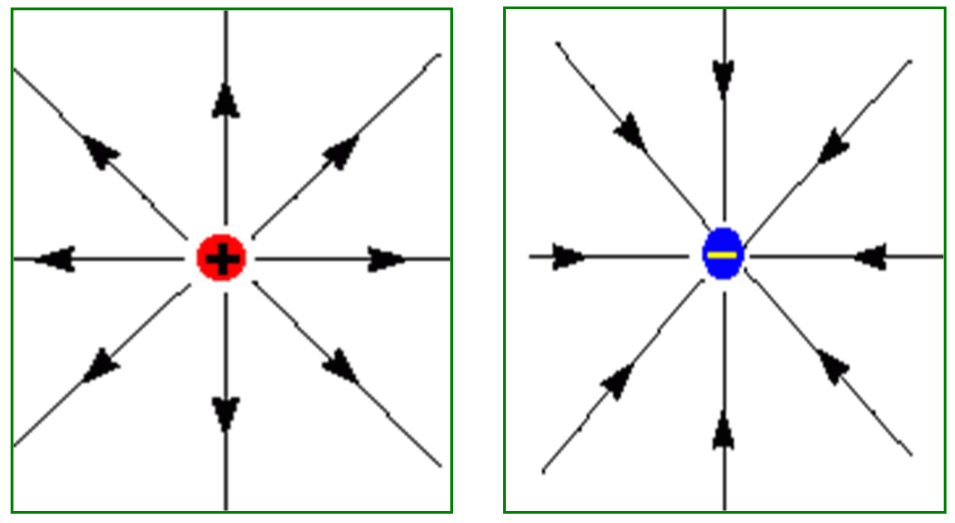
\includegraphics[width=0.80\textwidth]{Elektrisches Feld .png}
    \caption{Links nach außen gerichteter Feldvektor, rechts nach innen gerichteter Feldvektor.}
\end{figure}
Elektrische Feldlinien starten an positiven und enden an negativen Ladungen. 
Bei gleichen Ladungen stoßen sich die Feldlinien ab, bei entgegengesetzten Ladungen enden sie in der negativen Ladung.
Feldlinien können niemals bei der Ladung enden von der sie herkommen (keine geschlossenen Feldlinien).
\begin{figure}[H]
    \centering
    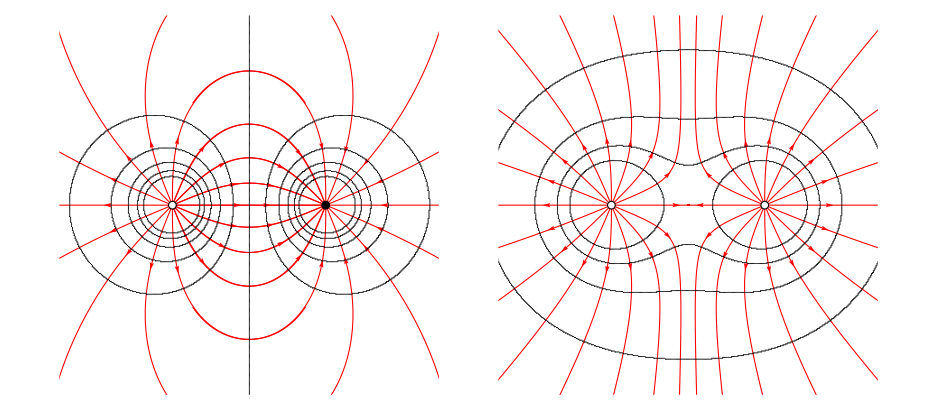
\includegraphics[width=0.80\textwidth]{Elektrisches Feld Ladungen.png}
    \caption{Links zwei entgegengesetzt Ladungen, Rechts zwei identische Ladungen}
\end{figure}

\subsection{Elektrische Leiter in einem elektrischen Feld}
Das Elektrische Feld im inneren eines geschlossenen Leiters ist immer null.
An der Oberfläche eines Leiters steht das elektrische Feld immer senkrecht zur Oberfläche.
Ein Beispiel für diese Eigenschaften ist der Faraday-Käfig.
\begin{figure}[H]
    \centering 
    \includegraphics[width=0.50\textwidth]{faraday käfig.png}
    \caption{Zu sehen ist, dass im inneren des Leiters das Elektrische Feld Null ist und die Feldlinien senkrecht zur Oberfläche stehen.}
\end{figure}

\subsection{Das Superpositionsprinzip}
Will man ein Elektrisches Feld für mehrere Ladungen berechen, so ergibt sich das resultierende Feld und Kraft 
durch die Überlagerung der einzel Felder.
Für das Elektrische Feld der Ladungen $q_i$ am Punkt $P$ (die Probeladung) gilt:
\begin{align}
    E_\mathrm{P}=k\cdot \sum_{i=1}^n \frac{q_i}{|\vec{r_i}|^2}\hat{r_i}
\end{align}
Die Kraft auf die Probeladung $q$ ergibt sich dann als:
\begin{align}
    \vec{F}=q\vec{E}_\mathrm{P}
\end{align}


\subsection{Spannung}
Die elektrische Spannung ist Arbeit im elektrischen Feld. Ihre Einheit ist $[\vec{E}]=\frac{\mathrm{V}}{\mathrm{m}}$.
Die Ladung q befindet sich in einem elektrischen Feld $\vec{E}(\vec{r})$ und soll von $\vec{r_1}$ nach $\vec{r_2}$ verschoben
werden. Dafür ist die Arbeit:
\begin{align}
    W&=\int_{\vec{r_1}}^{\vec{r_2}}\vec{F}(\vec{r})\,d\vec{r}\\
    &=q\int_{\vec{r_1}}^{\vec{r_2}}\vec{E}(\vec{r})\,d\vec{r}
\end{align}
notwendig.\\

\noindent Der Ausdruck des Integrals des Elektrischen Feldes wird als Potentialdifferenz ($U_2-U_1$) bezeichnet:
\begin{align}
    \int_{\vec{r_1}}^{\vec{r_2}}\vec{E}(\vec{r})\,d\vec{r}=U_2-U_1
\end{align}
Somit ergibt sich für die Arbeit $W$ im elektrostatischen Feld:
\begin{align}
    W&=q\int_{\vec{r_1}}^{\vec{r_2}}\vec{E}(\vec{r})\,d\vec{r}=q(U_2-U_1)
\end{align}
Die Arbeit in einem elektrostatischen Feld ist vom Weg unabhängig und hängt
nur vom Anfangspotential \( U_1 \) und Endpotential \( U_2 \) ab.
Ist dies gegeben, so handelt es sich um ein \textbf{konservatives Kraftfeld}.\\

\noindent In einem solchen Feld existiert ein Potential \( U(\vec{r}) \), aus dem das elektrische Feld berechnet werden kann:
\begin{align}
\vec{E}(\vec{r}) = -\vec{\nabla} U(\vec{r})
\end{align}

Diese Gleichung beschreibt, wie stark und in welche Richtung sich das Potential ändert.
Das \textbf{Minuszeichen} zeigt an, dass das elektrische Feld in Richtung des stärksten Abfalls des Potentials zeigt.\\

\noindent Das Potential einer Punktladung $Q$ lässt sich über 
\begin{align}
    U(\vec{r})=k\cdot\frac{Q}{r}\, \left(+U_0\right)
\end{align}
berechnen.\\

\noindent Die Spannung (Potentialdifferenz) ist nur definiert zwischen zwei Punkten.
Für die Potentialdifferenz zwischen Punkt $A$ und Punkt $B$ gilt:
\begin{align}
    U_{AB}=U(\vec{r_2})-U(\vec{r_1})=\frac{Q}{4\pi\varepsilon_0}\left(\frac{1}{r_2}-\frac{1}{r_1}\right)
\end{align}
Ist das Potential gleich Null, so liegt der Punkt im unendlichen. 
\begin{align}
    \lim_{r\to\infty}U(\vec{r})=0
\end{align}
Also: umso weiter weg man von einer Punktladung geht, desto kleiner wird das Potential.

\subsection{Plattenkondensator}
\begin{figure}[H]
    \centering
    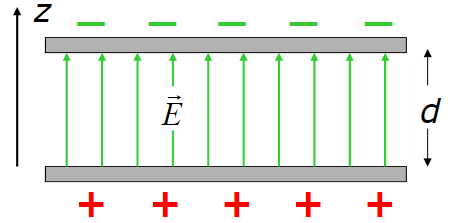
\includegraphics[width=0.6\textwidth]{Plattenkondensator.png}
    \caption{Der Aufbau eines Plattenkondensators mit der $z$-Achse}
\end{figure}
Bei einem Plattenkondensator gibt es zwei parallele, gegengesetzt geladene Metallplatten im Abstand $d$.
Diese bilden einen Kondensator aus.
Die Feldvektoren stehen senkrecht auf der positiv geladenen Platte und sind senkrecht auf die negative Platte gerichtet.
Sie entsprechen dem Einheitsvekor in $z$-Richtung:
\begin{align}
    \vec{E}\,||\,\hat{e}_z
\end{align}
Zudem ist das Elektrische Feld konstant, also homogen (überall gleich stark und gleiche Richtung) im inneren des Kondensators.
\begin{align}
    \vec{E}(\vec{r})=\vec{E}_0=const.\label{Plattenkondensator homogen}
\end{align}
Die Potenzialdifferenz (Spannung) zwischen den Platten ist:
\begin{align}
    \Delta U&=\int_0^d E(z)\,dz\\
    &=E_0\int_{0}^{d}dz\label{E_0 rausziehen}\\
    &=E_0\cdot d
\end{align}
Schritt~\ref{E_0 rausziehen} geht auf Grund des homogenen Feldes innerhalb des Plattenkondensators (siehe Formel~\ref{Plattenkondensator homogen}).
Für das Feld folgt damit:
\begin{align}
    E_0=\frac{\Delta U}{d}
\end{align}
Für die Einheit des elektrischen Feldes gilt $[E]=\frac{\mathrm{V}}{\mathrm{m}}$.
Bei Platten endlicher länge, ist das Feld am Rand (also Rechts und links) inhomogen.

\subsubsection{Beweis für die homogenität des elektrischen Feldes des Plattenkondensators}
Man betrachte eine Probeladung $q$ die sich im Abstand $a$ über einer großen Fläche mit 
gleichmäßiger Flächenladungsdichte $\sigma$ befindet.\\
Diese Fläche trägt eine Ladung:
\begin{align}
    dQ=\sigma\cdot da
\end{align}
Die Probeladung spürt eine Kraft durch das elektrische Feld dieser Fläche.
\begin{align}
    dF=k\cdot\frac{q\cdot dQ}{b^2}=k\cdot \frac{q\cdot \sigma\cdot dA}{b^2}
\end{align}
dabei ist $b$ der Abstand zwischen Probeladung und einem infinitesimal kleinen Flächenelement $dA$.\\

\noindent Nun zerlegt man die Kraft in zwei Richtungen. 
Einmal senkrecht zur Fläche (wirksame Kaft)
\begin{align}
    dF_s=dF\cdot \cos \alpha
\end{align}
und einmal Parallel zur Fläche (Symmetrische Kraft, diese hebt sich auf.)
\begin{align}
    dF_p=dF\cdot \sin \alpha=0
\end{align}
Die Symmetrische Kraft hebt sich auf, da alle horizontalen Anteile der Kräfte von gegenüberliegenden
Flächenelementen kompensiert werden.\\

\noindent Nun wird ein Ring mit Radius $r$ und Breite $dr$ betrachtet. Für die Fläche gilt:
\begin{align}
    dA=2\pi r\,dr
\end{align}
Es gelten folgende Beziehungen:
\begin{align}
    r=a\cdot\tan\alpha\\
    b=\frac{a}{\cos\alpha}
\end{align}
Die Ableitung von $r$ nach $\alpha$:
\begin{align}
    \frac{dr}{d\alpha}=\frac{a}{\cos^2\alpha}
\end{align}
Eingesetzt in $dF_s$ mit anschließendem Umformen und Integrieren gibt:
\begin{align}
    F=\frac{q\cdot \sigma}{2\varepsilon_0}
\end{align}
Somit haben wir bewiesen, dass die Kraft unabhängig von $a$ ist und somit konstant ist.
Somit ist das Feld eines idealen Plattenkondensators homogen.\\

\noindent Für die Kraft zweier Platten mit Ladung $Q$ gilt:
\begin{align}
    E=\frac{\sigma}{\varepsilon_0}=\frac{Q}{\varepsilon_0\cdot A}
\end{align}

\subsection{Kapazität}
Die Kapazität $C$ ist ein Maß dafür, wieviel Ladung man in einem Kondensator bei konstanter Spannung speichern kann.\\
Für das elektrische Feld gilt:
\begin{align}
    E&=\frac{U}{d}\\
    &=\frac{Q}{\varepsilon_0A}
\end{align}
Die Kapazität $C$ ist nun das Verhältnis zwischen der Ladung $Q$ und der Spannung $U$
\begin{align}
    C&=\frac{Q}{U}\\
    &=\frac{A\varepsilon_0}{d}
\end{align}
Diese Kapazität $C$ hängt nur von der Geometrie ab.
Ihre Einheit ist Farad $[C]=1\,\mathrm{F}=1\frac{\mathrm{A\,s}}{V}$
\begin{figure}[H]
    \centering
    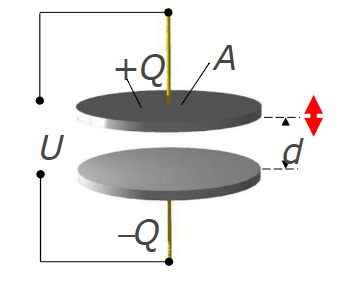
\includegraphics[width=0.40\textwidth]{aufbau plattenkondensator.png}
    \caption{Aufbau eines Plattenkondensators mit seinen relevanten Größen.}
\end{figure}

\subsection{Schaltzeichen eines Plattenkondensators}
\begin{figure}[H]
    \centering
    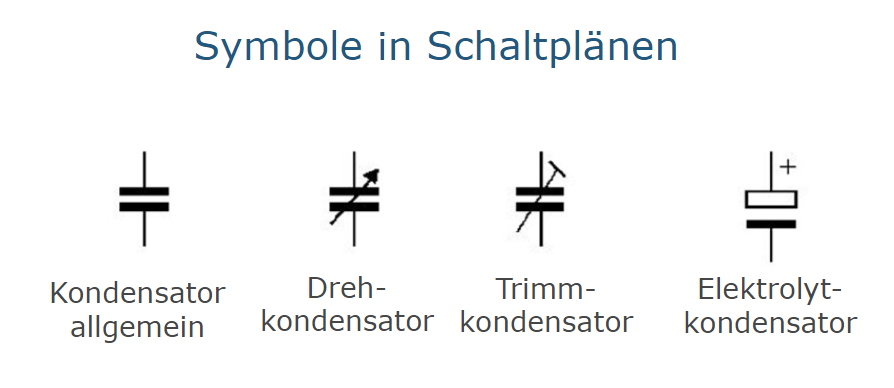
\includegraphics[width=0.8\textwidth]{Plattenkondensator schaltplan.png}
\end{figure}

\subsection{Der elektrische Dipol}
Zwei Unterschiedliche Ladungen im Abstand $d$ nennt man elektrischer Dipol.
Das Dipolmoment $\vec{p}$ ist definiert als:
\begin{align}
    \vec{p}=q\vec{d}
\end{align}
Das Dipolmoment ist ein Vektor, entlang der Verbindungslinie der beiden Ladungen.
$\vec{d}$ ist immer der Vektor von der negativen Ladung zur positiven. $q$ ist der Betrag einer der
beiden Ladungen (Diese sind beim Dipolmoment identisch).
\begin{enumerate}
    \item Permanentes Dipolmoment:\\
    Im \ce{HCl}-Molekül haben das \ce{H+} und das \ce{Cl-} einen Abstand $d$ und eine Ladung $q=e$.\\
    Für das Dipolmoment ergibt sich somit:
    \begin{align}
        \vec{p}=e\vec{d}
    \end{align}
    \item Induziertes Dipolmoment:\\
        Ein äußeres Feld verschiebt positive und negative Ladungsschwerpunkte.
        Ein Beispiel ist das Xenon Atom. Hier gilt:
        \begin{align}
            &\vec{d}\propto \vec{E}\\
            &\vec{p}\propto \vec{E}
        \end{align}
    \item Kompliziertere Ladungsverteilungen können in erster Näherung als Dipol angesehen werden. Als Beispiel ist hier 
    das Wasser Molekül zu nennen.
    \begin{figure}[H]
        \centering
        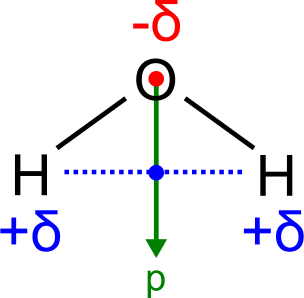
\includegraphics[width=0.3\textwidth]{Dipole_Water.png}
        \caption{Wasser Molekül mit Dipolmoment}
    \end{figure}
\end{enumerate}

\subsubsection{Homogenes elektrisches Feld}
Ein homogenes elektrisches Feld ist ein Feld, in dem die elektrische Feldstärke überall gleich groß und gleich gerichtet ist.\\
Auf eine positive ($q$) und eine negative ($-q$) Ladung $q$ wirkt das elektrische Feld $\vec{E}$.
Die Kräfte die auf Ladung 1 und Ladung 2 wirken ergeben sich durch:
\begin{align}
    \vec{F}_1&=q\vec{E}\\
    \vec{F}_2&=-q\vec{E}
\end{align}
Die resultierende Kraft auf den Dipol ist:
\begin{align}
    \vec{F}_\mathrm{Dipol}&=\vec{F}_1+\vec{F}_2\\
    &=q\vec{E}-q\vec{E}\\
    &=\vec{0}
\end{align}
Der Dipol bleibt jedoch nicht in Ruhe. Es wirkt ein Drehmoment:
\begin{align}
    \vec{M}_\mathrm{Dipol}&=\vec{r}_1\times \vec{F}_1+\vec{r}_1\times \vec{F}_2\\
    &=q\vec{r}_1\times \vec{E}-q\vec{r}_2\times\vec{E}\\
    &=q(\vec{r}_1-\vec{r}_2)\times\vec{E}\\
    &=q \vec{d}\times \vec{E}\\
    &\text{Mit dem Dipolmoment}\ \vec{p}=q\vec{d}\notag\\
    &=\vec{p}\times \vec{E}
\end{align}
Ein Dipol in einem homogenen elektrischen Feld erfährt ein Drehmoment,
das ihn so ausrichtet, dass sein Dipolmoment parallel zum elektrischen Feld zeigt.
Sobald diese Ausrichtung erreicht ist, bleibt der Dipol in dieser Stellung,
weil dann kein Drehmoment mehr auf ihn wirkt.
\begin{figure}[H]
    \centering
    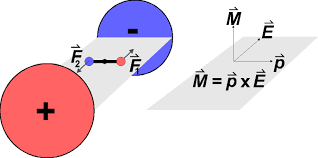
\includegraphics[width=0.80\textwidth]{Dipol im elektrischen Feld.png}
    \caption{Ein Dipol mit zwei Ladungen (kleine Punkte rot/blau) im Elektrischen Feld mit den vom Elektrischen Feld auf die Ladung wirkenden Kräfte.}
\end{figure}


\subsubsection{Inhomogenes elektrisches Feld}
Ein inhomogenes elektrisches Feld bedeutet, $\vec{E}(\vec{r})$ ist nicht überall gleich (also homogen) sondern je nach Ort Unterschiedlich.
Somit ist die Kraft die auf die Ladung wirkt nicht gleich groß, weil das elektrische Feld inhomogen ist.
\begin{align}
    \vec{F}_1&=q\vec{E}(\vec{r}_1)\\
    \vec{F}_2&=-q\vec{E}(\vec{r}_2)
\end{align}
Die Gesamtkraft des Dipols ergibt sich als:
\begin{align}
    \vec{F}_\mathrm{Dipol}&=\vec{F}_1+\vec{F}_2\\
    &=q\vec{E}(\vec{r}_1)-q\vec{E}(\vec{r}_2)\\
    &\not=\vec{0}
\end{align}
Diese ist nicht gleich dem Nullvektor, da $E(\vec{r}_1)\not=\vec{E}(\vec{r}_2)$.
Es existiert im gegensatz zum homogenen elektrischen Feld eine \textbf{resultierende Kraft}, also eine Translationskraft.\\

\noindent Für kleine Dipole, also $d\to 0$ kann die elektrische Feldstärke entwickelt werden. 
Für eine Dimension (also alle Vektoren sind Parallel) gilt:
\begin{align}
    E_2=E_1-\frac{dE}{dx}d
\end{align}
Diese Kraft hängt von der Änderung des elektrischen Felds $\frac{dE}{dx}$ und der Größe des Dipolmoments $p=qd$ ab.

\subsection{Dielektrikum}
Bringt man zwischen die Platten eines Kondensators eine isolierende Platte, so sinkt die Spannung $U$ um den Faktor $\varepsilon$.
Da die Ladung $Q=C\cdot U=const$ ist, muss sich die Kapazität $C$ um den Faktor $\varepsilon$ erhöhen.
\begin{align}
    C_\mathrm{Dielektrikum}=\varepsilon C_\mathrm{Vakuum}=\varepsilon\varepsilon_0\frac{A}{d}
\end{align}
mit der relativen Dielektrizitätskonstante $\varepsilon>1$.
Isolierende Stoffe heißen deshalb auch \textbf{Dielektrika}.


\subsection{Der elektrische Strom}
\subsubsection{Bewegte Ladungen in Feldern}
Ein Teilchen mit einer Ladung $q$ erfährt im elektrischen Feld die Kraft:
\begin{align}
    \vec{F}_E=q\,\vec{E}
\end{align}
Hierdurch wird diese beschleunigt. Nach dem 2. Newtonschen Gesetz gilt:
\begin{align}
    \vec{F}=\dot{\vec{p}}=m\ddot{\vec{r}}
\end{align}
Die Beschleunigung erfolgt in Richtung der Feldlinien.\\
Die Bewegunsgleichung ergibt sich durch gleichsetzen und Umformen:
\begin{align}
    \ddot{\vec{r}}=\frac{q}{m}\vec{E}
\end{align}
\vspace{0.5cm}

\noindent Ein Beispiel für bewegte Ladungen ist die Oszillographenröhre (Auch Braunsche Röhre).
Dies ist eine von Ferdinand Braun entwickelte Rähre. An der Kathode werden Elektronen 
durch Erhitzung erzeugt, an der Anode werden die Elektronen beschleunigt und an den Ablenkplatten wird ein elektrisches 
Feld erzeugt, welches zur Ablenkung des Elektronenstrahls dient. Auf einem Leuchtschirm sind die Auftreffpunkte 
der Elektronen sichtbar.

\subsubsection*{Physikalische Beschreibung der Brownschen Röhre}
\begin{itemize}
\item Ladung: $q_e=-e$
\item Masse: $m=m_e$
\end{itemize}
Das Elektrische Feld ist definiert als:
\begin{align}
    \vec{F}=q\cdot \vec{E}
\end{align}
Mit dem 2. Newtonschen Gesetz und der Ladung $q=e$ folgt:
\begin{align}
    F=m_e\cdot a_e=e\cdot E_a
\end{align}
Umstellen nach der Beschleunigung $a_e$ gibt:
\begin{align}
    a_e=\frac{e}{m_e}E_a
\end{align}
Mit $E_a=\frac{U_a}{d}$ folgt:
\begin{align}
    a_e=\frac{eU_a}{m_ed}\label{a_e}
\end{align}
Für $a=const$ gilt:
\begin{align}
    d=\frac{1}{2}a_et^2
\end{align}
Umstellen auf $d$ gibt:
\begin{align}
    t=\sqrt{\frac{2d}{a_e}}
\end{align}
Mit Gleichung~\ref{a_e} folgt:
\begin{align}
    t=\sqrt{\frac{2m_ed^2}{eU_a}}\label{t_e}
\end{align}
Da es sich um eine eindimensionale Bewegung mit $a=const$ handelt gilt für die Geschwindigkeit:
\begin{align}
    v=a_e\cdot t=\frac{e}{m_e}E_at=\sqrt{\frac{2eU_a}{m_e}}
\end{align}

\subsubsection*{Ablenkung durch die Platten}
In den Platten wirkt die transversale Kraft.
\begin{align}
    F_p=ma_p=eE_p=e\frac{U_p}{h}
\end{align}
Daraus folgt die Transversalbeschleunidung $a_p$ mit:
\begin{align}
    a_p=\frac{eU_p}{m_eh}
\end{align}
Die Ablenkung $z$ ergibt sich aus der Kinematik für $a_p=const$:
\begin{align}
    z=\frac{1}{2}a_pt_p^2
\end{align}
Die Flugzeit durch die Platten $t_p$ ergibt sich aus der länge der Platten $l$ und der Geschwindigkeit $v$:
\begin{align}
    t_p=\frac{l}{v}=l\sqrt{\frac{m_e}{2eU_a}}
\end{align}
Damit den Termen für $a_p$ und $t_p$ berechnet sich die Ablenkung $z(U_p)$ als:
\begin{align}
    z(U_p)&=\frac{eU_p}{2m_eh}l^2\frac{m_e}{2eU_a}\\
    &=\frac{U_pl^2}{4U_ah}
\end{align}

\vspace{0.5cm}
\noindent Die Braunsche Röhre kann als Oszilloskop zur Messung schneller Signale verwendet werden.

\subsection{Das Ohmsche Gesetz:}
Die Spannung $U$ erzeugt in einem Leiter ein homogenes Elektrisches Feld $E$.
Dies führt zu einem Strom $I$ durch die Fläche A.\\
Die Stromdichte $j$ ist definiert als:
\begin{align}
    j=\frac{I}{A}
\end{align}
Die Stärke des Stromes ist proportional zum angelegten elektrischen Feld $E$:
\begin{align}
    \vec{j}=\sigma \vec{E}
\end{align}
Mit der Leitfähigkeit $\sigma$. Sie ist eine spezifische Materialkonstante. Ihre Einheit ist:
\begin{align}
    [\sigma]=\frac{\mathrm{A}}{\mathrm{Vm}}=\frac{1}{\mathrm{(V/A)m}}
\end{align}
Das Verhältnis aus angelegter Spannung $U$ zum Strom $I$ nennt man den Widerstand $R$:
Es gilt:
\begin{align}
    R=\frac{U}{I}
\end{align}
Mit $[R]=\mathrm{V/A}=1\Omega$ also Ohm.\\

\noindent Das homogene elektrische Feld führt zu einer Potentialdifferenz zwischen den Leiter-Enden.
\begin{align}
    \varphi_2-\varphi_1=U&=\int_{0}^{l}E\, dr\\
    &=E\cdot l\\
    &=\frac{j}{\sigma}l\\
    &=\frac{l}{\sigma}\cdot \frac{I}{A}
\end{align}
$A$ ist die Querschnittsfläche und $l$ die Länge des Leiters. Daraus folgt:
\begin{align}
    U=\frac{l}{\sigma A}I
\end{align}
Mit dem Widerstand
\begin{align}
    R=\frac{l}{\sigma A}
\end{align}
Also ergibt sich:
\begin{align}
    U=R(U,I,T,...)\cdot I
\end{align}
Der Wiederstand kann von Unterschiedlichen Größen abhängen.
Bei vielen Leitern ist der Widerstand praktisch konstant.\\
Dann gilt das Ohm'sche Gesetz:
\begin{align}
    \boxed{U=R\cdot I}\qquad (R=const)
\end{align}

\subsection{Ohmsche Widerstände}
Widerstände sind durch 4 oder 5 Farbringe gekennzeichnet. Aus diesen Ringen können die spezifischen Eigenschaften 
wie der Wiederstand $R$ und die Toleranz ermittelt werden.

\subsection{Parallelschaltung zweier Widerstände}
\begin{figure}[H]
    \centering
    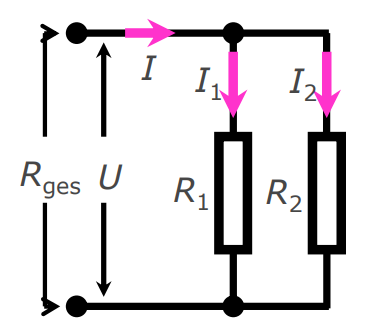
\includegraphics[width=0.4\textwidth]{parallelschaltung.png}
\end{figure}
Der Gesamtstrom ist:
\begin{align}
    I_\text{ges}=I_1+I_2
\end{align}
Nach dem Ohmschen Gesetz folgt:
\begin{align}
    I_\text{ges}=U\left(\frac{1}{R_1}+\frac{1}{R_2}\right)
\end{align}
Mit 
\begin{align}
    R_\text{ges}=\frac{U}{I_\text{ges}}
\end{align}
folgt:
\begin{align}
    R_\text{ges}=\frac{R_1\cdot R_2}{R_1+R_2}
\end{align}
Für $N$ Wiederstände gilt:
\begin{align}
    \frac{1}{R_\text{ges}}=\sum_{i=1}^{N}\frac{1}{R_i}
\end{align}

\subsection{Serienschaltung von Widerständen}
\begin{figure}[H]
    \centering
    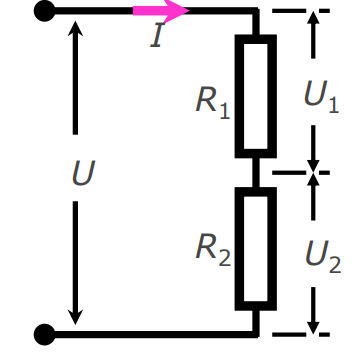
\includegraphics[width=0.4\textwidth]{serienschaltung.png}
\end{figure}
Für die Spannung gilt:
\begin{align}
    U=U_1+U_2
\end{align}
Außerdem gilt:
\begin{align}
    U_i=R_i\cdot I
\end{align}
Somit folgt:
\begin{align}
    U=I(R_1+R_2)=I\cdot R_\text{ges}
\end{align}
Somit gilt:
\begin{align}
    R_\text{ges}=R_1+R_2
\end{align}
Für $N$ Wiederstände in Serienschaltung gilt:
\begin{align}
    R_\text{ges}?\sum_{i=1}^{N}R_i
\end{align}

\subsection{Netzwerke und Kirchhoff'sche Regeln}
$\Rightarrow$ Berechnung von Spannung und Strömen in beliebigen Netzwerken.
\subsubsection{Kirchhoffsche Regeln}
\begin{enumerate}
    \item Die Knotenregel:\\
        Aufgrund von Ladungserhaltung fließt soviel Strom in einen Knoten wie auch wieder herausfließt.
        Im Knoten verschwindet die Summe aller Ströme:
        \begin{align}
            \sum_{i=1}^{I_i}=0
        \end{align}
        \begin{figure}[H]
            \centering
            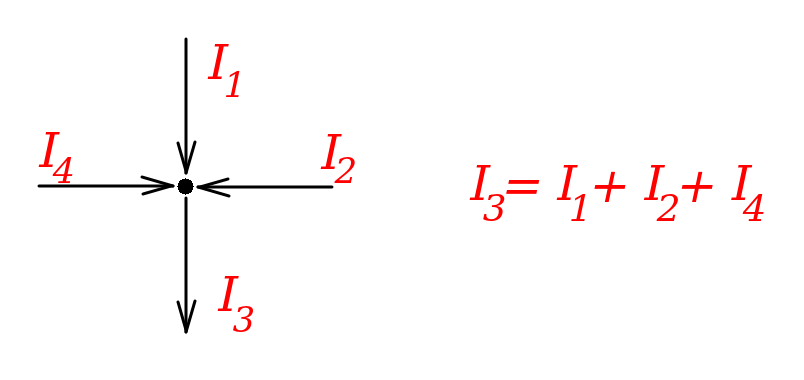
\includegraphics[width=0.5\textwidth]{knotenregel.png}
            \caption{Grafik zur Knotenregel}
        \end{figure}
    \item Die Maschenregel:\\
        In jeder geschlossenen Masche verschwindet die Summe aller Spannungen
        \begin{align}
            \sum_{i=1}^{N}U_i=0
        \end{align}
        \begin{figure}[H]
            \centering
            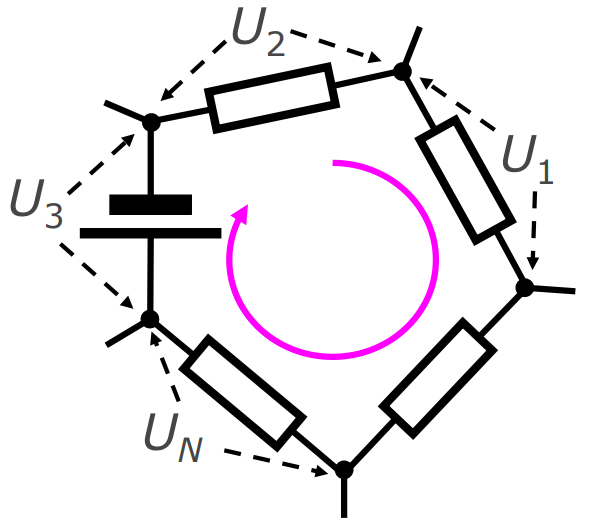
\includegraphics[width=0.4\textwidth]{Maschenregel.png}
            \caption{Grafik zur Maschenregel}
        \end{figure}
\end{enumerate}

\subsection{Spannungsteiler}
Ein \textbf{Spannungsteiler} ist eine Schaltung aus mindestens zwei Widerständen in Reihe, die eine Eingangsspannung $U$ aufteilt. An jedem Widerstand fällt ein Teil der Spannung ab – je nachdem, wie groß der Widerstand ist.

\vspace{1em}

\noindent \textbf{Ziel:} Wir wollen z.\,B. aus einer hohen Spannung (z.\,B. 9 V) eine kleinere Spannung erzeugen (z.\,B. 3 V).

\subsubsection*{1. Unbelasteter Spannungsteiler}
Ein Unbelasteter SPannungsteiler ist ein Spannungsteiler ohne Verbraucher.
\begin{figure}[H]
    \centering
    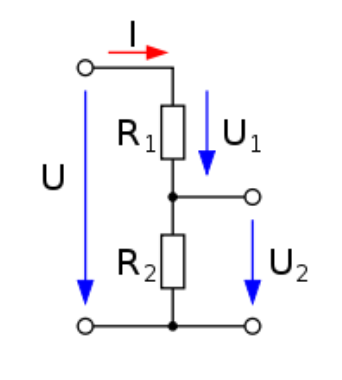
\includegraphics[width=0.3\textwidth]{spannungsteiler 1.png}
    \caption{Schaltplan für einen Unbelasteten Spannungsteiler}
\end{figure}

\textbf{Gesamtstrom:}
\begin{align}
    I =\frac{U}{R_\text{ges}}= \frac{U}{R_1 + R_2}
\end{align}



\textbf{Spannung an $R_2$:}
\begin{align}
U_2 &= \frac{U}{R_\text{ges}}\cdot R_2\\
  \frac{U_2}{U}  &=\frac{R_2}{R_1+R_2}
\end{align}

\textbf{Verhältnisformel:}
\begin{align}
    \frac{R_1}{U_1}=\frac{R_2}{U_2}
\end{align}

\subsubsection*{2. Belasteter Spannungsteiler}
Ein belasteter Spannungsteiler ist ein Spannungsteiler mit einem Verbraucher.
Wenn man einen Verbraucher (z.\,B. Lampe, Sensor) mit Widerstand $R_L$ anschließt, beeinflusst das den Spannungsteiler. Der Widerstand $R_2$ und $R_L$ wirken dann wie ein \textbf{Parallelwiderstand}.

\begin{figure}[H]
    \centering
    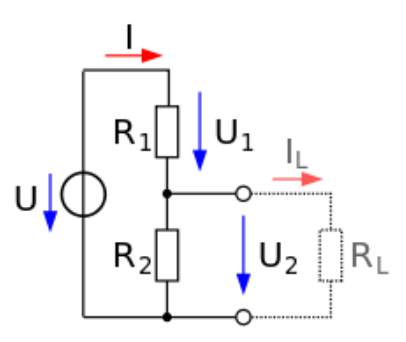
\includegraphics[width=0.3\textwidth]{spannungsteiler 2.png}
    \caption{Schaltplan für einen belasteten Spannungsteiler}
\end{figure}

\noindent \textbf{Parallele Kombination:}
\begin{align}
    R_P = \frac{R_2 \cdot R_L}{R_2 + R_L}
\end{align}
\textbf{Neue Spannung am Lastwiderstand:}
\begin{align}
    U_2 = U \cdot \frac{R_P}{R_1 + R_P}
\end{align}

\vspace{2em}
\noindent Der Verbraucher „belastet“ die Schaltung, wodurch $U_2$ kleiner wird als ohne Last.\\
Ein Spannungsteiler ist also eine Methode eine Spannung aufzuteile, jedoch ist diese Methode empfindlich gegenüber angeschlossenen Verbrauchern.

\subsection{Wheatstonsche Brücke}
%Vorlesung 4 Folie 8


\subsection{Parallelschaltung von Kondensatoren}
\begin{figure}[H]
    \centering
    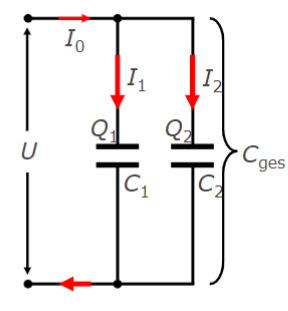
\includegraphics[width=0.3\textwidth]{Parallelschaltung von Kondensatoren.png}
\end{figure}
Für jeden einzelnen Kondesator gilt
\begin{align}
    Q_1=C_1U\qquad Q_2=C_2U
\end{align}
Die Gesamtladung auf den Kondensatorplatten ist
\begin{align}
    Q_\text{ges}&=Q_1+Q_2\\
    &=C_1U+C_2U\\
    &=(C_1+C_2)U\\
    &=C_\text{ges}U
\end{align}
Daraus folgt $C_\text{ges}=C_1+C_2$.\\
Verallgemeinerung auf $N$ parallel geschaltete Kondensatoren ergibt
\begin{align}
    C_\text{ges}=\sum_{i=1}^{N}C_i
\end{align}

\subsection{Serienschaltung von Kondensatoren}
\begin{figure}[H]
    \centering
    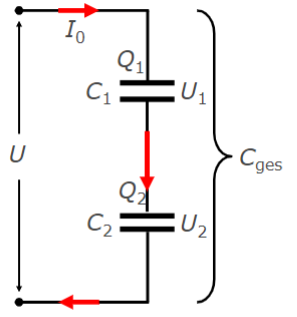
\includegraphics[width=0.3\textwidth]{Serienschaltung von Kondensatoren.png}
\end{figure}
Für jeden Kondensator gilt jetzt (mit $q_1=Q_2=Q$)
\begin{align}
    Q=C_1U_1\qquad Q=C_2U_2
\end{align}
Die Gesamtspannung setzt sich aus Einzelspannungen zusammen 
\begin{align}
    U&=U_1+U_2\\
    &=\frac{Q}{C_1}+\frac{Q}{C_2}\\
    &=Q\left(\frac{1}{C_1}+\frac{1}{C_2}\right)\\
    &=Q\frac{1}{C_\text{ges}}
\end{align}
Daraus folgt $\frac{1}{C_\text{ges}}=\frac{1}{C_1}+\frac{1}{C_2}$.\\
Verallgemeinerung auf $N$ in Serie geschaltete Kondensatoren ergibt
\begin{align}
    \frac{1}{C_\text{ges}}=\sum_{i=1}^{N}\frac{1}{C_i}
\end{align}

\subsection{Laden und Entladen von Kondensatoren}
\begin{figure}[H]
    \centering
    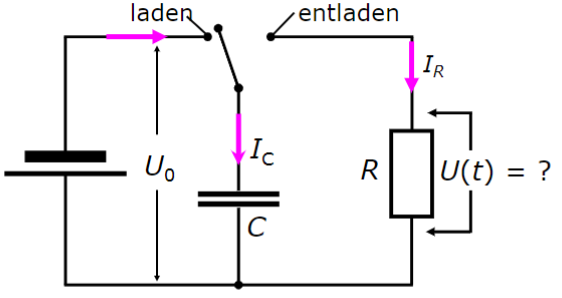
\includegraphics[width=0.5\textwidth]{Laden und entladen von Kondensatoren.png}
\end{figure}
Zunächst wird der Kondensator über einen Schalter mit einer Batterie verbunden
und lädt sich dabei auf die Spannung $U_0$ auf. Danach wird umgeschaltet,
so dass der Strom über $I_R$ abfließt.\\

\noindent Es soll nun die Spannung $U(t)$ berechnet werden,
die über einen Kondensator der Kapazität $C$ beim Aufladen über einen Widerstand $R$ 
abfällt.\\
Der Strom durch den Kondensator ist 
\begin{align}
    I(t)=\frac{U_0-U(t)}{R}
\end{align}
Gleichzeitig gilt
\begin{align}
    \frac{d Q}{dt}=I(t)=C\frac{dU(t)}{dt}
\end{align}
Daraus ergibt sich durch Gleichsetzen eine Differentialgleichung für $U(t)$
\begin{align}
    C\frac{dU(t)}{dt}=\frac{U_0-U(t)}{R}
\end{align}
Dies lässt sich umformen zu 
\begin{align}
    \frac{dU(t)}{dt}+\frac{1}{RC}U(t)=\frac{U_0}{RC}
\end{align}
Die Lineare DGL 1. Ordnung mit konstanten Koeffizienten, jetzt aber inhomogen.\\

\noindent Die Lösung der homogenen Gleichung lautet 
\begin{align}
    U_h(t)=A\exp\left(-\frac{t}{RC}\right)
\end{align}
Eine partikuläre Lösung $U_p(t)$ ergibt sich leicht aus der Bedingung
\begin{align}
    \lim_{t\to\infty} U_p(t)=U_0
\end{align}
Also gilt für die Gesamtlösung
\begin{align}
    U(t)&=U_p(t)+U_h(t)\\
    &=U_0+A\exp\left(-\frac{t}{RC}\right)
\end{align}
Die konstante $A$ ist mit der Anfangsbedingung $U(t)=0$ für
$t=0$ festgelegt.
\begin{align}
    U(0)=U_0+A=0\quad \Leftrightarrow \quad A=-U_0
\end{align}
Damit ergibt sich die gesuchte Aufladekurve eines Kondensators
\begin{align}
    U(t)=U_0\left[1-\exp\left(-\frac{t}{RC}\right)\right]
\end{align}
Aus $Q=CU$ folgt
\begin{align}
    \frac{dQ_c}{dt}=I_C=-C\frac{dU}{dt} \quad \text{und}\quad T_R=\frac{U}{R}
\end{align}
Da beim Entladen $I_C=I_R$ ist, folgt
\begin{align}
    &\frac{dU(t)}{dt}=-\frac{1}{RC}U(t)\\
    \Rightarrow &\frac{dU(t)}{dt}+\frac{1}{RC}U(t)=0
\end{align}
Lineare, homogene DGL 1. Ordnung mit konstanten Koeffizienten
für die Funktion $U(t)$. Die Lösung lautet 
\begin{align}
    U(t)=U_0\exp\left(-\frac{t}{RC}\right)
\end{align}
$U_0$ ist die Spannung zum Zeitpunkt $t=0$. $U(t)$ und damit auch der Entladestrom
$I_R(t)=U(t)/R$ klingen exponentiell ab mit Zeitkonstanten
\begin{align}
    \tau=RC
\end{align}
Mit der Einheit $[\tau]=\SI{1}{\frac{V}{A}\frac{A s}{V}}=\SI{1}{s}$.
\begin{align}
    U(t)=U_0\exp\left(-\frac{t}{\tau}\right)
\end{align}
\begin{align}
    U(t)=\frac{U_0}{R}\exp\left(-\frac{t}{\tau}\right)
\end{align}


%Vorlesung 5
\newpage
\section{Magnetostatik}
Während statische Ladungen von elektrischen Feldern umgeben sind, sind magnetische Materialien
(z.B. Eisen) von Magnetfeldern umgeben.\\
Ein Magnet ist ein Dipol. Im Gegensatz zu elektrischen Ladungen, die einzeln
auftreten können, gibt es keine einzelnen Magnetpole. Starke Permanent-Magnete sind zum Beispiel \ce{Nd2Fe14B}.\\

\noindent Fließende Ladungen, also Ströme in einem Leiter erzeugen Magnetfelder.
\begin{figure}[H]
    \centering
    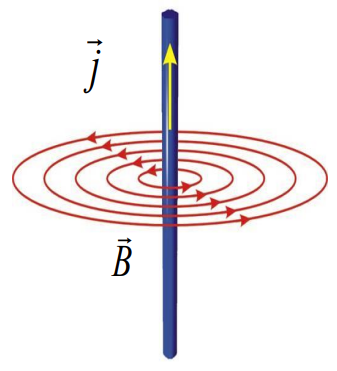
\includegraphics[width=0.4\textwidth]{Magnetfeld.png}
    \caption{Ein Stromdurchfließender Leiter bildet ein Magnetfeld.}
\end{figure}
\noindent Im Gegensatz zu elektrischen Feldlinien sind Magnetfeldlinien immer geschlossen.
Die Feldlinien geben Kraftwirkung (Richtung und Stärke) des Magnetfeldes an.
Die Richtung der Magnetfeldlinien kann einfach mit der rechten Hand demonstriert werden.
Dabei zeigt der Daumen in Richtung des Stroms uns die Gekrümmten Finger geben die Richtung des Magnetfeldes an.
\begin{figure}[H]
    \centering
    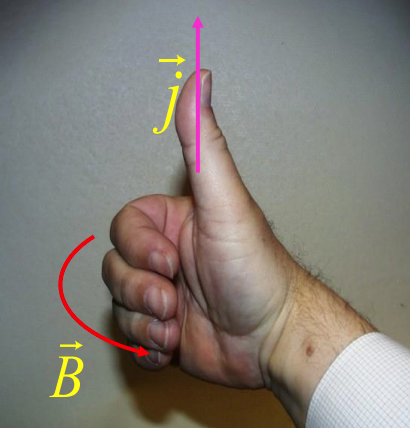
\includegraphics[width=0.4\textwidth]{rechte Hand.png}
    \caption{Mit der rechten Hand Regel kann die Richtung des Magnetfeldes ermittelt werden.}
\end{figure}
Das Magnetfeld eines geraden Leiters durch den der Strom $I$ fließt wird beschrieben durch
\begin{align}
    \vec{B}(\vec{r})=B(r)\cdot \vec{e}_\varphi.
\end{align}
Das Feld kann nur vom Abstand $r$ des Leiters abhängen. Die Feldlinien sind konzentrische Kreise.
$\vec{e}_\varphi$ ist der Einheitsvektor in Polarkoordinaten. Experimentel findet man für den 
Betrag von $B(r)$
\begin{align}
    B(r)\propto \frac{I}{r}.
\end{align}
Mit der Proportionalitätskonstante $\frac{\mu_0}{2\pi}$ ist das Magnetfeld eines stromdurchflossenden
Leiters daher
\begin{align}
    \vec{B}(\vec{r})=\frac{\mu_0}{2\pi}\frac{I}{r}\vec{e}_\varphi.
\end{align}
Hierbei ist zu beachten:
\begin{enumerate}
    \item $\mu_0$ ist die magnetische Permeabilität des Vakuums. Sie wird auch als magnetische Feldkonstante bezeichnet.
    Ihr Wert ist $\mu_0=4\pi\cdot\SI{ e-7}{\frac{V s}{A m}}$. Die Einheit des Magnetfelds ist damit $[\vec{B}]=\SI{1}{\frac{V s}{m^2}}=\SI{1}{T}$, also Tesla.
    \item In Materie muss die Formel für das Magnetfeld eines Leiters abgeändert werden. Mit der Permeabilität $\mu$ des Mediums gilt
    \begin{align}
        \vec{B}(\vec{r})=\frac{\mu_0\mu}{2\pi}\frac{I}{r}\vec{e}_\varphi.
    \end{align}
    Das heißt $\mu_0$ muss durch das Produkt $\mu_0\cdot \mu$ ersetzt werden.
    \item Der Leiter ist hier als unendlich ausgedehnt angenommen worden. Deswegen fällt das Feld nur wie $\frac{1}{r}$ ab und nicht gemäß $\frac{1}{r^2}$ wie im Falle von elektrischen Punktladungen.
\end{enumerate}

\subsection{Das Ampère'sche Gesetz}
Das Magnetfeld eines graden stromdurchflossenden Leiters lässt sich Verallgemeinern.
Das Resultat 
\begin{align}
    \vec{B}(\vec{r})=\frac{\mu_0}{2\pi}\frac{I}{r}\vec{e}_\varphi
\end{align}
lässt sich Umformen zu 
\begin{align}
    \vec{B}(\vec{r})2\pi r=\mu_0 I \vec{e}_\varphi,\\
    \vec{B}(\vec{r})\cdot \vec{e}_\varphi 2\pi r=\mu_0 I
\end{align}
Das $\vec{B}(\vec{r})$ nur eine $\varphi$-Komponente hat, entspricht dies einem Wegintegral entlang der kreisförmigen Schleife mit Radius $r$ um den Leiter
\begin{align}    
\boxed{\oint \vec{B}(\vec{r})\, d\vec{r}=\mu_0 I}
\end{align}
Das Wegintegral über das Vektorfeld $\vec{B}(\vec{r})$ entlang des Kreises mit dem Radius $r$, der den Strom $I$ umfasst ist $\mu_0 I$.\\

\noindent Die Gleichung bedeutet anschaulich, dass (stationäre) Ströme (statische) magnetische Felder hervorrufen.
Magnetfelder werden generell durch das Fließen von Strömen erklärt.
Das bedeutet z.B. dass in einem magnetischen Stück Eisen mikroskopische Ströme fließen.
Das Wegintegral in der Gleichung darf entlang jeder beliebig geformten geschlossenen Kurve, die den Strom $I$ umschließt berechnet werden.

\subsection{Magnetfeld einer langen stromdurchflossenen Spule}
Das Magnetfeld einer Spule entsteht dadurch, dass die Feldlinien der einzelnen Leiter nach der Rechten handregel im Querschnitt unterschiedlich Laufen. So 
läuft das Feld durch das Innere der Spule.
\begin{figure}[H]
    \centering
    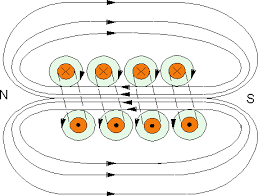
\includegraphics[width=0.5\textwidth]{Magnetfeld Spule.png}
    \caption{Im Querschnitt verläuft das Magnetfeld der Drahte von Oben im Uhrzeigersinn, da die Spannung ins Bild dort hineingeht (rechte Handregel). Bei den unteren Drähten kommt der Strom aus dem Bild raus also verläuft das Feld gegen den Uhrzeigersinn (rechte Hand). }
\end{figure}
Das Magnetfeld im Inneren einer Spule der Länge $l$ kann mit dem Ampère'schen Gesetz berechnet werden.
Näherungsweise gilt für das Magnetfeld innerhalb der Spule $\vec{B}=\vec{B}_0=\vec{const}$ und im Außenraum $\vec{B}=\vec{0}$.

\subsection*{Herleitung des Magnetfelds einer langen Spule}
\begin{figure}[H]
    \centering
    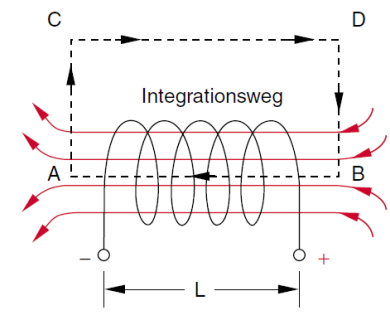
\includegraphics[width=0.5\textwidth]{Magnetfeld Spule Herleitung.png}
    \caption{Der Weg des Kreisintegrals wird aufgeteilt in innerhalb und außerhalb liegenden Teil der Spule.}
\end{figure}
\begin{align}
    \oint \vec{B}(\vec{r}) \cdot d\vec{r} &= \int_{A}^{B} dx + \oint \vec{B}(\vec{r}) \cdot d\vec{r} = \mu_0 N I \label{153}\\
    &= \vec{B} \cdot L \cdot \vec{e}_x + 0 = \mu_0 N I\label{154}
\end{align}
Das Integral im ersten Schritt wird in den Weg innerhalb der Spule und den Weg außerhalb der Süule aufgeteilt. Das Wegintegral außerhalb ist annähernd null.
Das Integral im inneren der Spule lässt sich lösen. Für $x$ wird $L\vec{e}_x$ eingesetzt, da $L$ die Länge von Strecke $x$ ist und diese in $x$-Richtung zeigen muss.
Nun kann die letzte Gleichung umgestellt werden und es folgt 
\begin{align}
    B=\mu_0\frac{N\cdot I}{L}
\end{align}
Diese Formel ist für dicht gewickelte Spulen mit großer Windungszahldichte $\frac{N}{L}$ sehr genau.

\subsection{Magnetfeld einer Spule mit Eisenkern}
Das Magnetfeld einer Spule vergrößert sich, wenn ein Eisenkern in die Spule geschoben wird.
Andere Materialien zeigen nahezu keinen Effekt oder verringern das Magnetfeld sogar.
Es gilt \begin{align}
    B=\mu_0\frac{N\cdot I}{l}
\end{align}
Mit Materie gilt aus $\mu_0$ wird $\mu_0\cdot \mu$ also 
\begin{align}
    B=\mu_0\mu\frac{N\cdot I}{l}
\end{align}
Da für Eisen $\mu=5000$ gilt ergibt sich die große Verstärkung mit dem Eisen-Kern.

%Folie: Dia-, Para-, Ferromagnete










\end{document}
